\documentclass[12pt,A4,titlepage]{article}
\usepackage[dvipsnames,rgb,dvips]{xcolor}
\usepackage{graphicx}
\usepackage{psfrag}
\usepackage{dcolumn}
\usepackage{bm}
\usepackage{amsmath}
\usepackage{amssymb}
\usepackage[rflt]{floatflt}
\usepackage{latexsym}
%\usepackage{float}
\usepackage{bm}
\usepackage{subcaption}
\usepackage{booktabs}
\usepackage{floatrow}
\floatsetup[table]{font=footnotesize}

\addtolength{\topmargin}{-1.9cm}
\addtolength{\textheight}{5.5cm}
\addtolength{\evensidemargin}{-1.2cm}
\addtolength{\oddsidemargin}{-1.2cm}
\addtolength{\textwidth}{2cm}
\pagestyle{myheadings}
\markright{{\small Jacopo Credi \hfill (910216-T396) \,}}
\DeclareMathOperator\erf{erf}
\author{Jacopo Credi}
\title{FFR135\\Artificial Neural Networks\\ \bigskip Examples sheet 1}

\usepackage{listings}
\usepackage{color} %red, green, blue, yellow, cyan, magenta, black, white
\definecolor{mygreen}{RGB}{28,172,0} % color values Red, Green, Blue
\definecolor{mylilas}{RGB}{170,55,241}
% Settings for writing Matlab code
\lstset{language=Matlab,%
	basicstyle=\small\ttfamily,
    %basicstyle=\color{red},
    breaklines=true,%
    morekeywords={matlab2tikz},
    keywordstyle=\color{blue},%
    morekeywords=[2]{1}, keywordstyle=[2]{\color{black}},
    identifierstyle=\color{black},%
    stringstyle=\color{mylilas},
    commentstyle=\color{mygreen},%
    showstringspaces=false,%without this there will be a symbol in the places where there is a space
    numbers=left,%
    numberstyle={\tiny \color{black}},% size of the numbers
    numbersep=9pt, % this defines how far the numbers are from the text
    %emph=[1]{for,end,break},emphstyle=[1]\color{red}, %some words to emphasise
    frame=single,                   % adds a frame around the code
  	rulecolor=\color{black},
    %emph=[2]{word1,word2}, emphstyle=[2]{style},    
}




\begin{document}
\parindent=0cm
\maketitle

\subsection*{Problem 1(a)}


\begin{figure}[H]
 \centering
    \begin{subfigure}[b]{0.32\textwidth}
        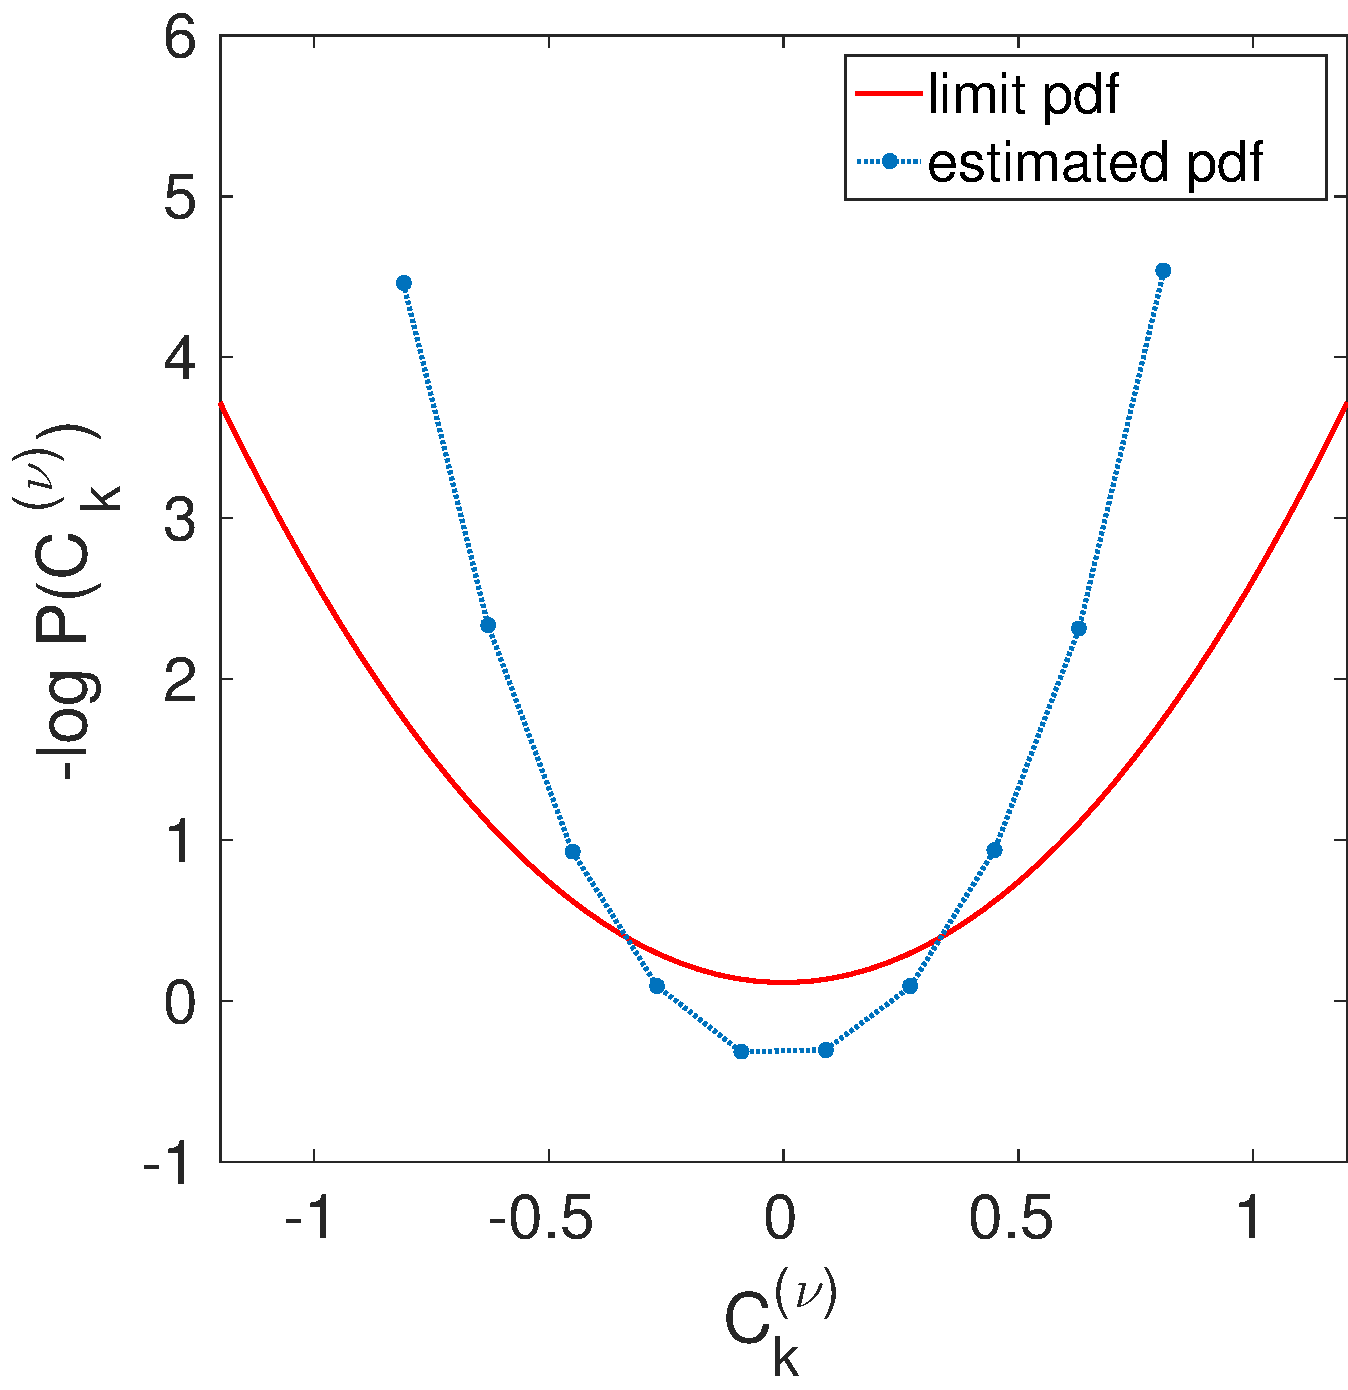
\includegraphics[width=\textwidth]{figures/fig_1a_1.pdf}
        \caption{$N = 10, \ p = 2$}
        \label{1a1}
    \end{subfigure}
    	\hfill
    \begin{subfigure}[b]{0.32\textwidth}
        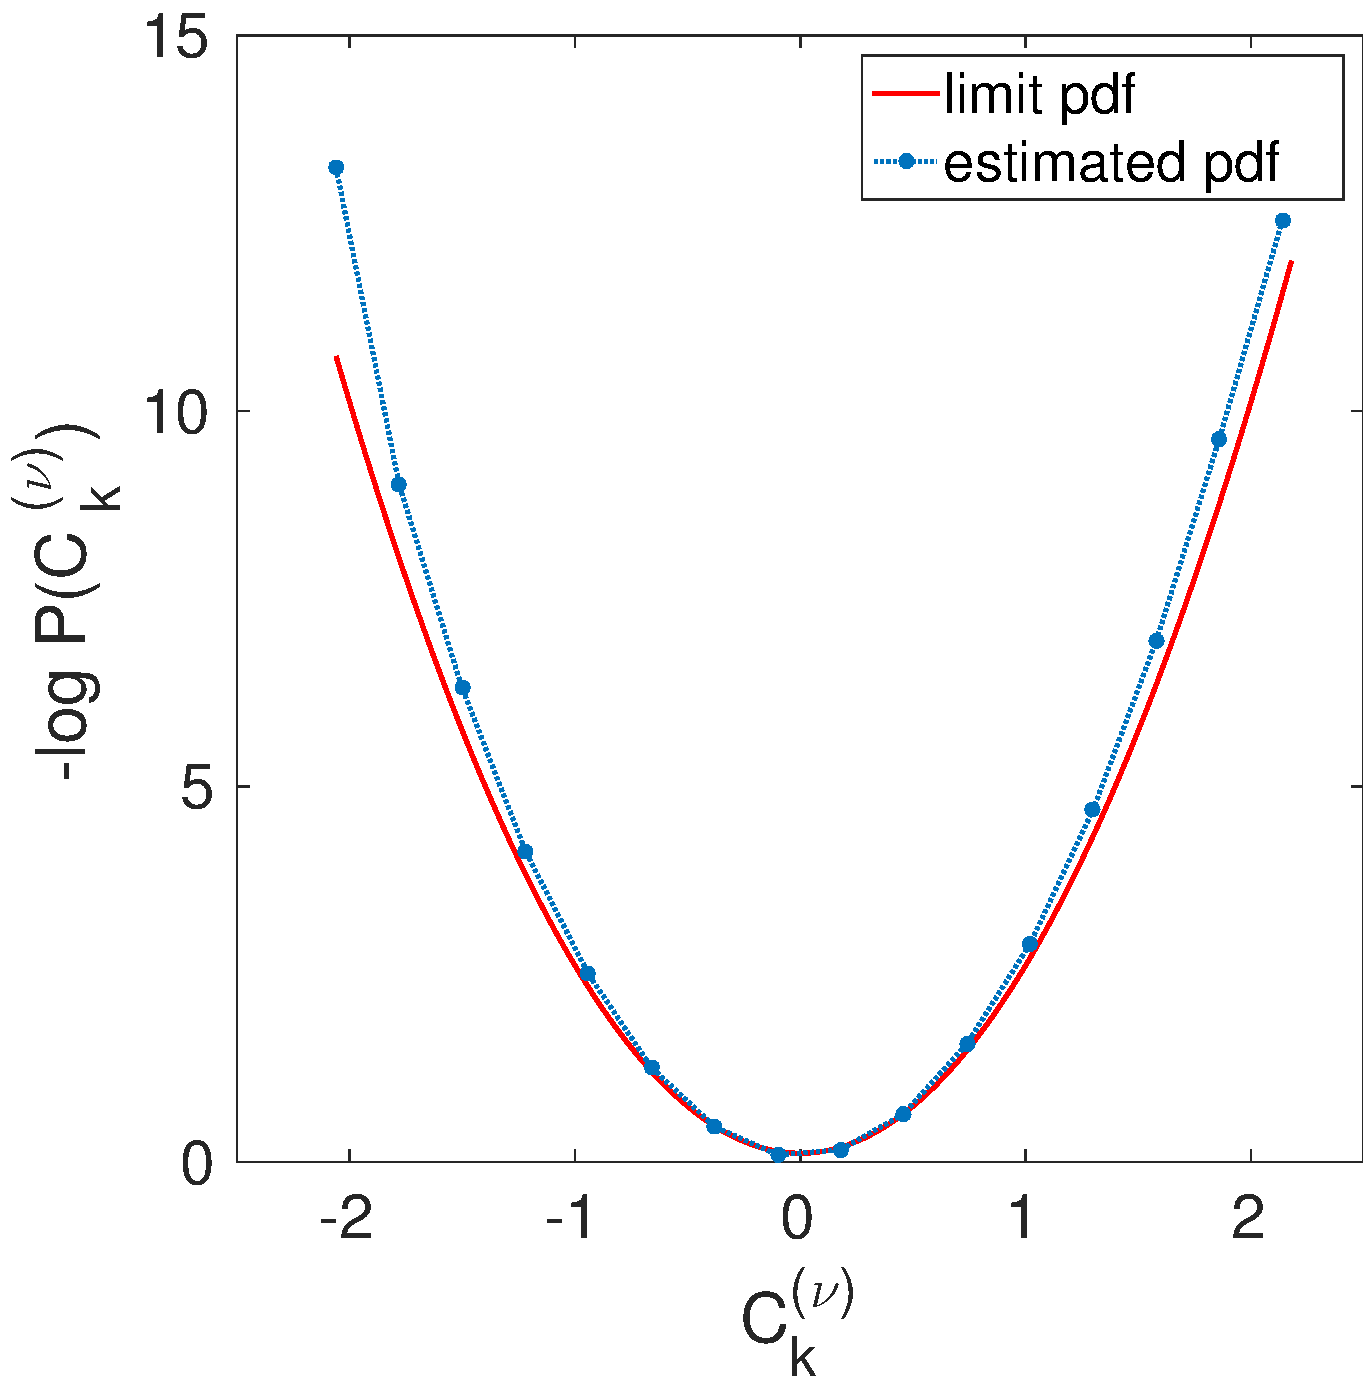
\includegraphics[width=\textwidth]{figures/fig_1a_2.pdf}
        \caption{$N = 50, \ p = 10$}
        \label{1a2}
    \end{subfigure}
    \hfill
    \begin{subfigure}[b]{0.32\textwidth}
        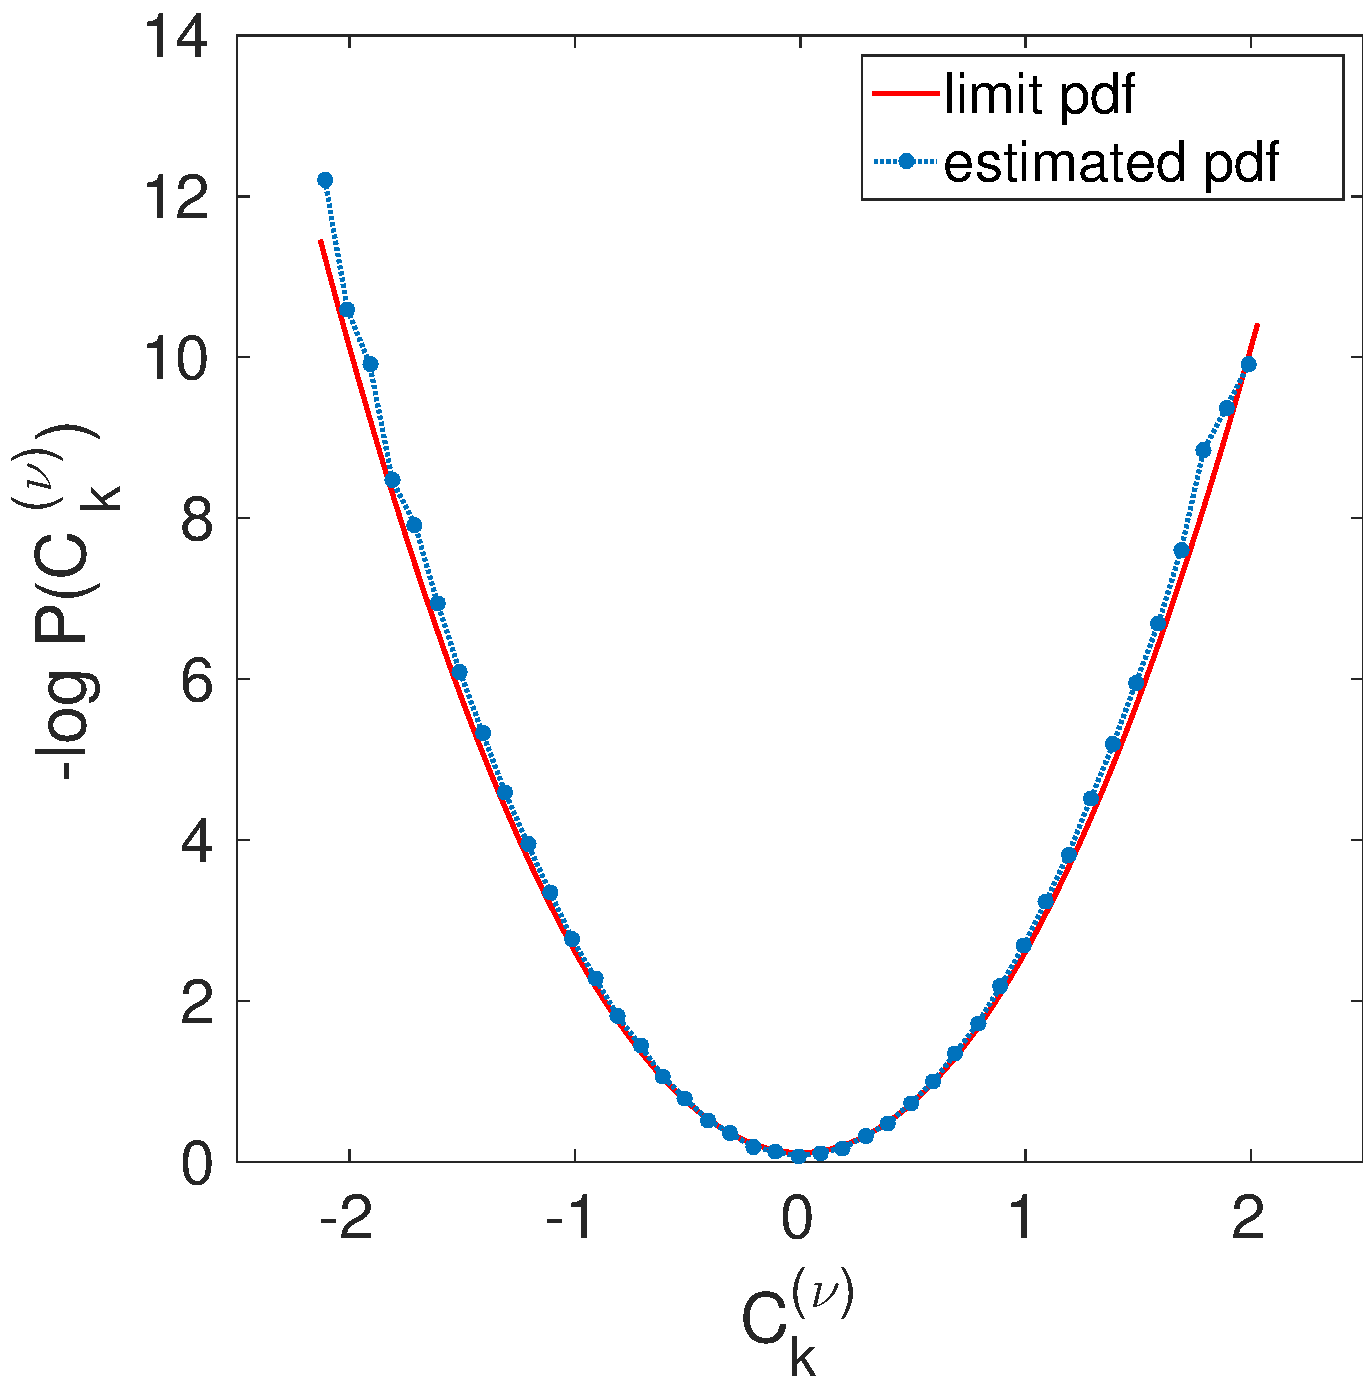
\includegraphics[width=\textwidth]{figures/fig_1a_3.pdf}
        \caption{$N = 100, \ p = 20$}
        \label{1a3}
    \end{subfigure}
    \caption{Blue dots and dashed line: numerically estimated pdf of the cross-talk terms in a deterministic synchronous Hopfield network. Red solid line: theoretical limit pdf.}
    \label{1a}
\end{figure}

\subsubsection*{Discussion}

A Hopfield network with synchronous deterministic update was implemented and used to numerically evaluate the distribution $P(C^{(\nu)}_k)$ of the cross-talk terms $C^{(\nu)}_k$ for different values of $N$ (number of bits) and $p$ (number of patterns).

In Fig. \ref{1a}, the obtained distributions are plotted and compared with the theoretical limit distribution
\begin{equation}
P(C^{(\nu)}_k) = \sqrt{\dfrac{N}{2 \pi p}} \exp\Bigl( - \dfrac{(C^{(\nu)}_k)^2}{2p / N}\Bigr) \ ,\qquad \text{valid for} \quad N \rightarrow \infty \ .
\end{equation}

Here, since the ratio $p/N$ is the same in the tree cases, the limit distribution is the same. Clearly, the agreement between the numerically estimated pdf and the limit pdf appears to increase as the number $N$ of bits increases.

For low values of $N$ (see e.g. the case $N = 10$), the distribution is taller and narrower than the limit distribution, suggesting that the single-step error probability, i.e. \\$P_{\textup{error}} = P(C^{(\nu)}_k > 1)$, is actually less than its corresponding theoretical value 
\begin{equation}
P_{\textup{error}}^{\textup{th}} = \frac{1}{2} \ \Bigl( 1 - \erf\bigl(\sqrt{\dfrac{N}{2p}}\bigr)\Bigr) \
\label{errorProb}
\end{equation}
in a deterministic Hopfield network of finite size, and tends to it as $N \rightarrow \infty$.
\subsubsection*{Reference code}
See \textsc{matlab} script \texttt{Exercise1a.m} and custom functions called in the script itself.


\clearpage

\subsection*{Problem 1(b)}

\begin{figure}[H]
\centering
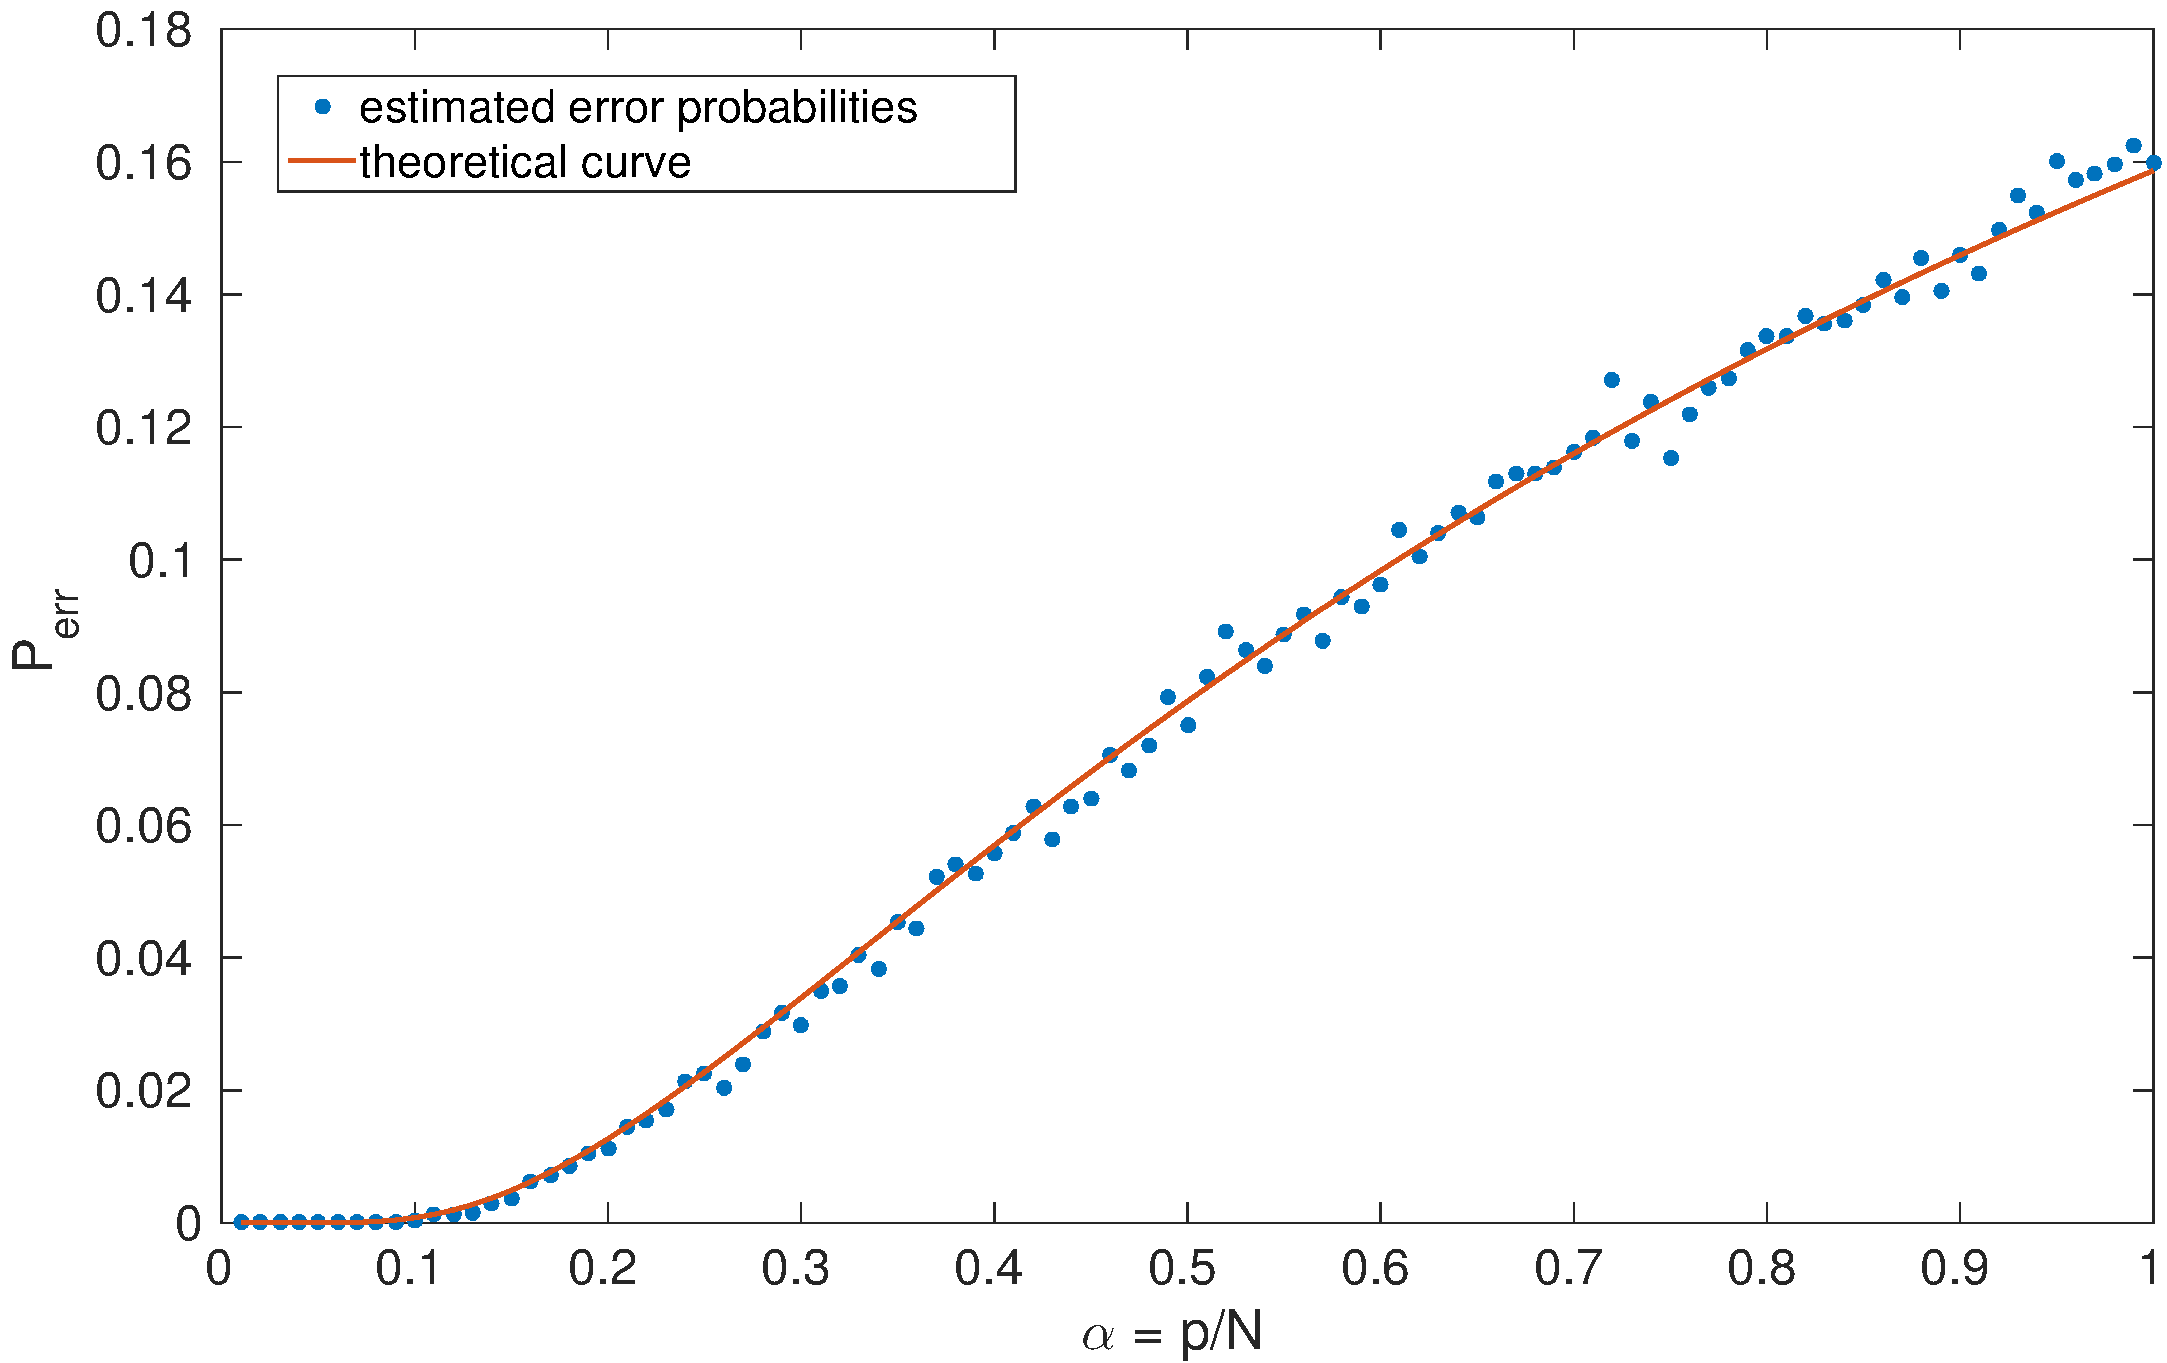
\includegraphics[width=0.9\textwidth]{figures/fig_1b.pdf}
\caption{Blue dots: estimated one-step error probabilities in a deterministic Hopfield network with $N = 100$ bits plotted against the ratio $p/N$. Red solid line: theoretical curve.}
\label{1b}
\end{figure}

\subsection*{Discussion}

Here, $P_{\textup{error}}(\alpha)$ was estimated by keeping the number $N$ of bits fixed ($N = 100$) and increasing the number of patterns by one, starting from $p=1$ and going up to $p = 100$.

For each value of $p$, the following procedure was repeated $M = 10000 $ times:
\begin{itemize}
\itemsep0em 
\item Generate $p$ random patterns and determine network weights using Hebb's rule.
\item Set the initial state to be pattern $\bm{\zeta}^{(1)}$ and perform a \textbf{single} network update step.
\item Check whether $s_1(t=1) = s_1(t=0)$. If not, then register an "error event''.
\end{itemize}
At the end of this simulation, $P_{\textup{error}}(\alpha)$ is estimated by
\[
P_{\textup{error}}^{\textup{est}} = \dfrac{\text{number of error events}}{M} \ .
\]
In Fig. \ref{1b}, the estimated probabilities are compared to the theoretical curve (see Equation~\ref{errorProb}), displaying a remarkably good agreement.

\subsubsection*{Reference code}
See \textsc{matlab} script \texttt{Exercise1b.m} and custom functions called in the script itself.
\clearpage

\subsection*{Problem 2(a)}

\begin{figure}[H]
\centering
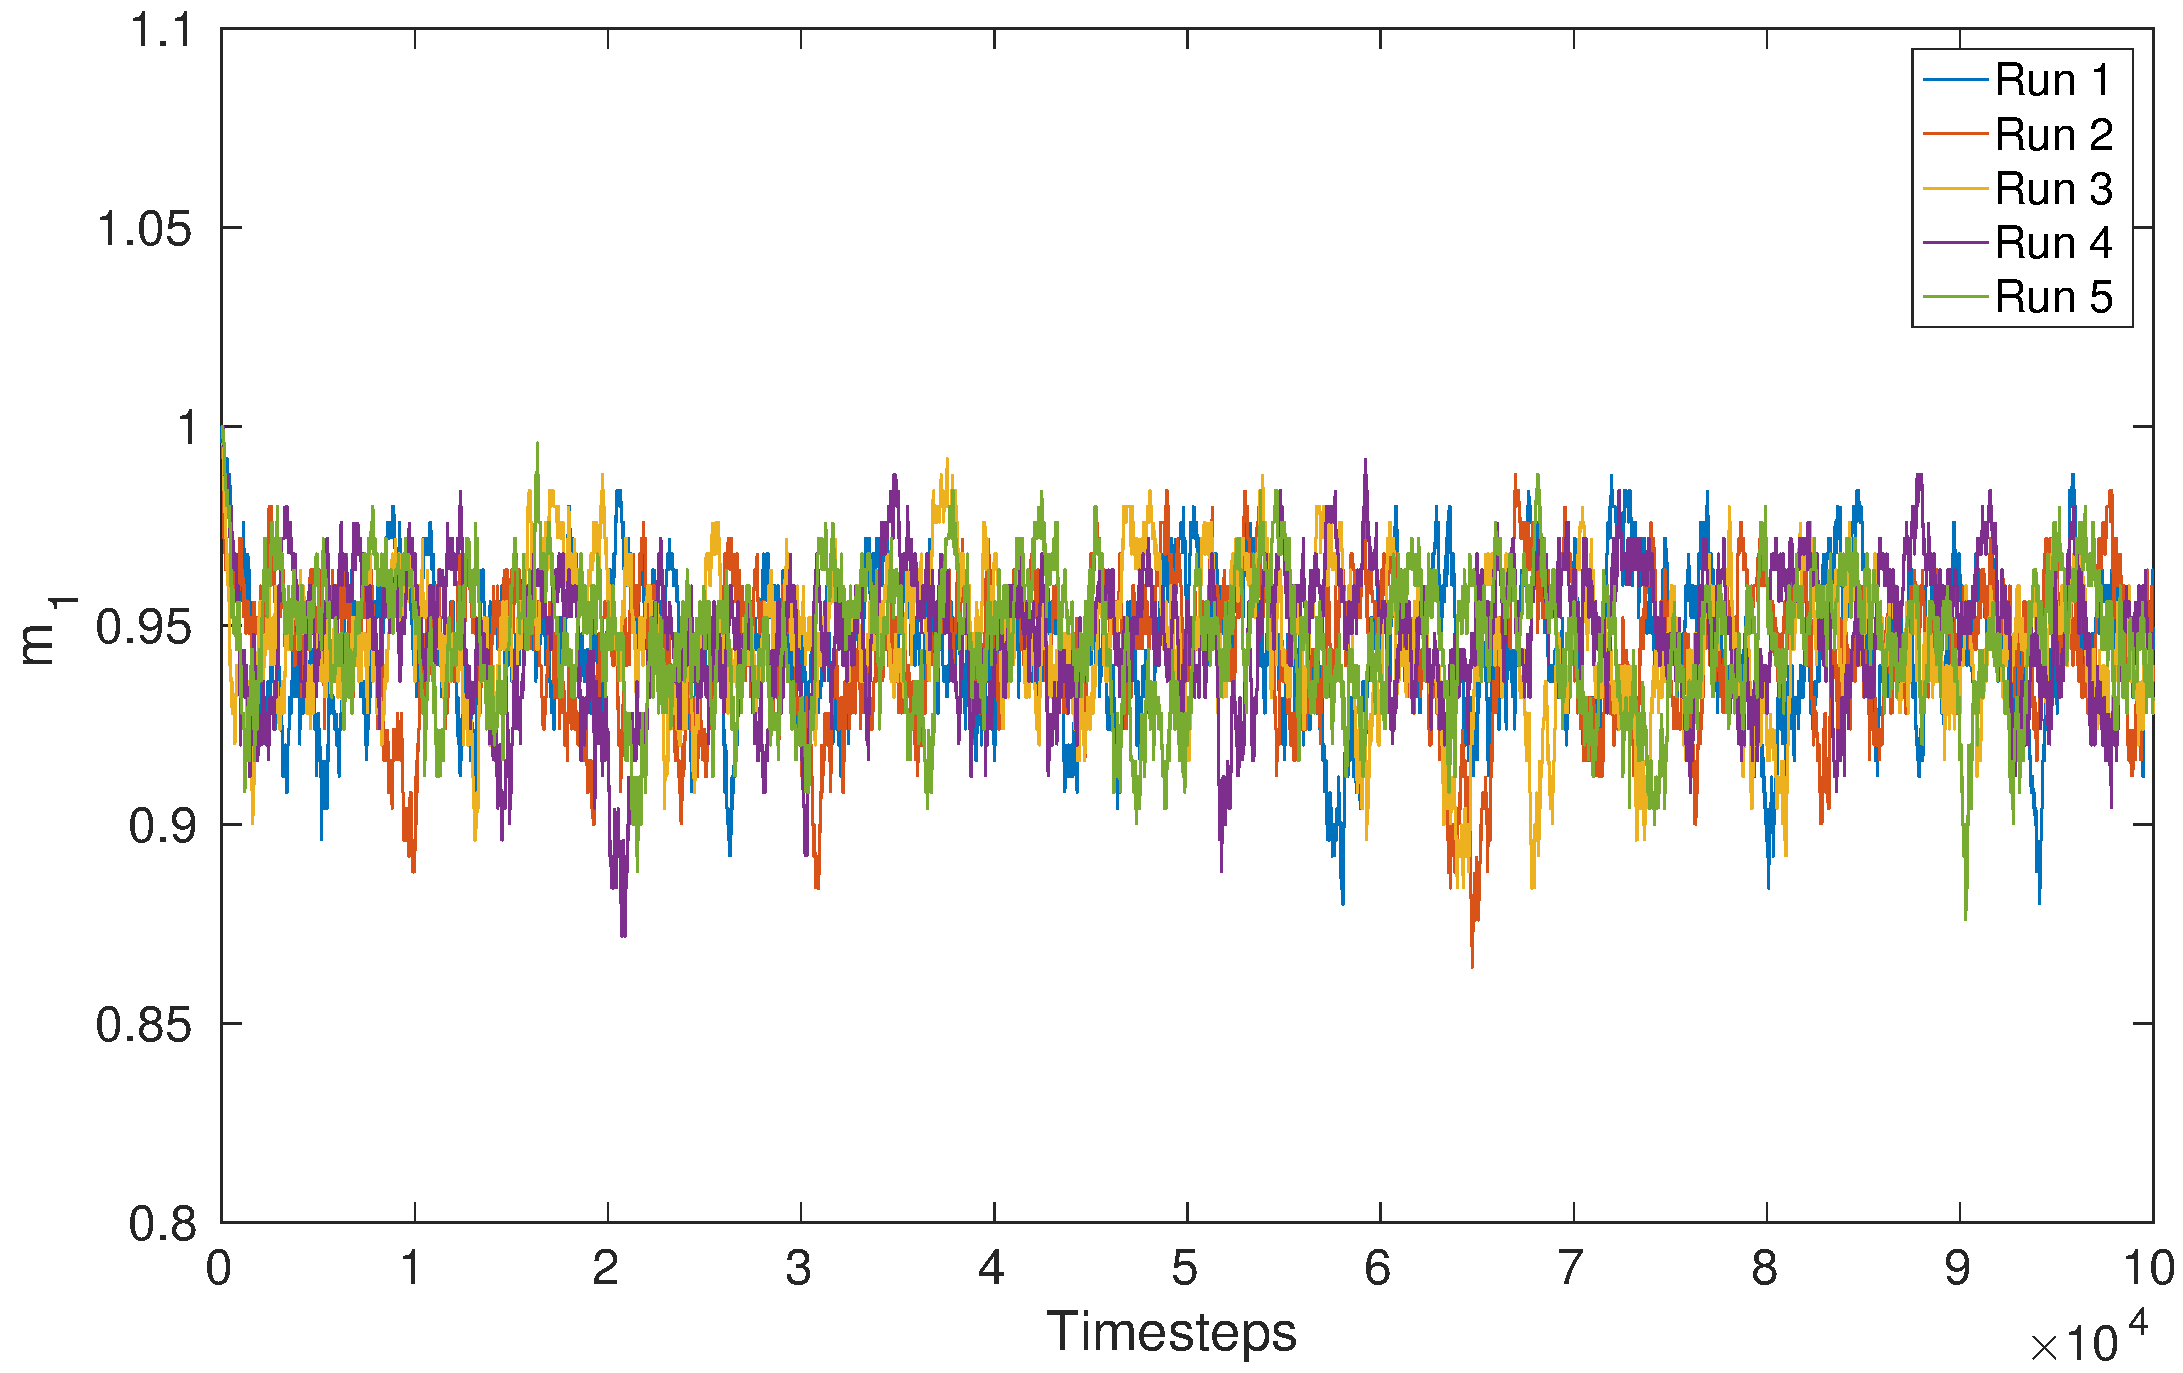
\includegraphics[width=\textwidth]{figures/fig_2a.pdf}
\caption{Evolution of a stochastic Hopfield network with $N = 500$ bits and $p = 10$ patterns. In all $5$ runs, the initial configuration is the  stored random pattern $\bm{\zeta}^{(1)}$ and the network is updated $10^5$ times. Noise level is fixed $\beta^{-1} = 0.5$.}
\label{2a}
\end{figure}

\subsection*{Discussion}
A Hopfield neural network with asynchronous stochastic updating was implemented and tested with a fixed noise level of $\beta^{-1} = 0.5$ and a load parameter $\alpha = 0.02$, corresponding to $N = 500$ bits and $p = 10$ patterns. 
The stored pattern $\bm{\zeta}^{(1)}$ is fed as initial configuration, and the network is then run for $10^5$ asynchronous updates. The whole process is repeated $5$ times. 

Fig.~\ref{2a} shows that at this noise and load level the initial pattern $\bm{\zeta}^{(1)}$ is stable, as the order parameter $m_1$ stabilises around a value of $0.95$. This suggests that in this point $(\beta^{-1}, \alpha)$ of the parameter space, the neural network can be used as a good memory device.

This simulation, however, does not allow us to give an estimate the burn-in time of the MCMC, as the equilibrium state is too close to the starting configuration.

\subsubsection*{Reference code}
See \textsc{matlab} script \verb!Exercise_2a_2b.m! and custom functions called in the script itself.
\clearpage

\subsection*{Ex. 2 (b)}

\begin{figure}[H]
\centering
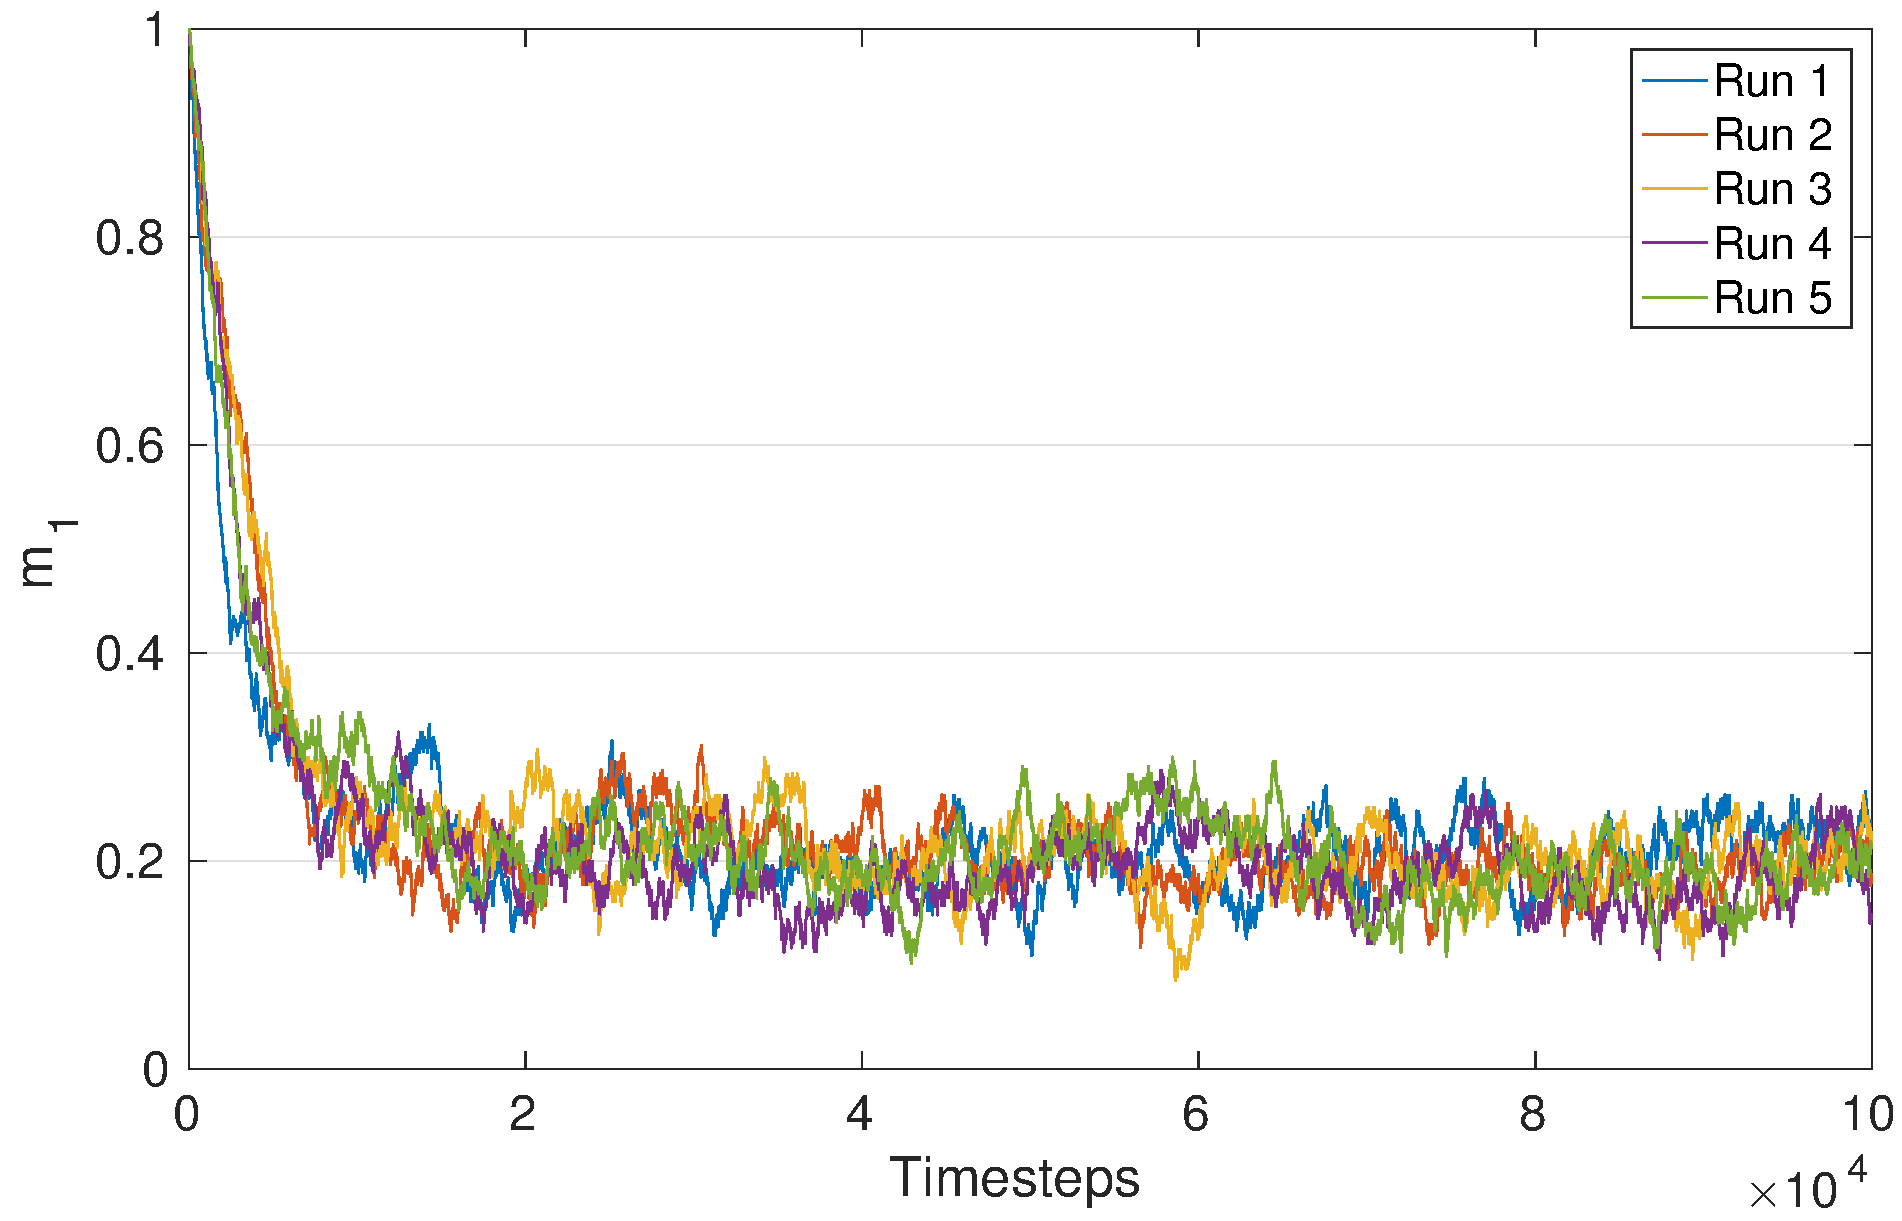
\includegraphics[width=\textwidth]{figures/fig_2b.pdf}
\caption{Evolution of a stochastic Hopfield network with $N = 500$ bits and $p = 100$ patterns. In all $5$ runs, the initial configuration is the stored random pattern $\bm{\zeta}^{(1)}$ and the network is updated $10^5$ times. Noise level is fixed $\beta^{-1} = 0.5$.}
\label{2b}
\end{figure}

\subsection*{Discussion}
In this second case, the number of stored pattern is increased to $p = 100 $, corresponding to a network load $ \alpha = 0.2 $. 

As predicted by the theory, the order parameter converges to a lower value than that of the previous case, as the network load is much higher. The theory predicts in fact that, when the noise is fixed, $\left<m_1(\alpha)\right>$ is a monotonically decreasing function of $\alpha$. 

With these parameters, the network cannot obviously be used as a memory device. However, the equilibrium value of the order parameter appears to be significantly different from zero, as the dimension of the network is finite. Some exploratory simulations with a much larger number of bits (up to $N = 10000$) showed that indeed the order parameter converges to zero for $ \alpha = 0.2 $.

Furthermore, Fig. \ref{2b} suggests that for these values of $\beta$, $N$ and $p$, a burn-in time of around 50000 iterates is sufficient to allow the system to reach the "thermal'' equilibrium.

\subsubsection*{Reference code}
See \textsc{matlab} script \verb!Exercise_2a_2b.m! and custom functions called in the script itself.
\clearpage

\subsection*{Ex. 3 (a)}


\begin{table}[H]
\centering
\resizebox{\textwidth}{!}{
\begin{tabular}{r|cccccc}
\toprule
$N = 500$ & $\alpha =0.025$ & $0.05$ & $0.1$ & $0.125$ & $0.15$ & $0.2$ \\ 
\midrule
$\beta^{-1} = 0.1$ & $1 \pm 2\cdot10^{-15}$ & $1\pm3\cdot10^{-6}$ & $1\pm3\cdot10^{-4}$ & $0.994\pm0.002$ &$0.05 \pm0.02$ & $0.238\pm0.005$ \\ 
$0.2$ & $1\pm4\cdot10^{-4}$ & $0.998\pm0.001$ & $0.958\pm0.008$ & $0.986 \pm 0.004$ & $0.11\pm0.11$ & $-0.2\pm0.02$ \\ 
$0.3$ & $0.996\pm0.001$ & $0.988\pm0.003$ & $0.971\pm0.004$ & $0.075\pm0.019$ & $-0.02\pm0.03$ & $0.2\pm0.2$ \\ 
$0.4$ & $0.980\pm0.003$ & $0.953\pm0.007$ & $-0.003\pm0.014$ & $0.11\pm0.07$ & $0.15\pm0.04$ & $0.12\pm0.02$ \\
$0.5$ & $0.943\pm0.006$ & $0.91\pm0.01$ & $0.02\pm0.03$ & $0.19\pm0.02$ & $0.07\pm0.02$ & $0.12\pm0.04$ \\
$0.6$ & $0.87\pm0.01$ & $0.06\pm0.07$ & $0.06\pm0.08$ & $0.10\pm0.02$ & $-0.01\pm0.03$ & $0.11\pm0.03$ \\
$0.7$ & $0.03\pm0.06$ & $0.11\pm0.03$ & $-0.06\pm0.13$ & $0.13\pm0.03$ & $0.0\pm0.1$ & $0.22\pm0.03$ \\
$0.8$ & $0.08\pm0.04$ & $0.01\pm0.10$ & $-0.05\pm0.03$ & $0.07\pm0.04$ & $0.02\pm0.14$ & $-0.06\pm0.10$ \\
\bottomrule
\end{tabular} 
}
\caption{Average value $\left<m_1\right>$ of the order parameter in equilibrium. N = 500.}
\label{table1}
\end{table}

\begin{table}[H]
\footnotesize
\centering
\resizebox{\textwidth}{!}{
\begin{tabular}{r|cccccc}
\toprule
$N = 1000$ & $\alpha =0.025$ & $0.05$ & $0.1$ & $0.125$ & $0.15$ & $0.2$ \\ 
\midrule
$\beta^{-1} = 0.1$ & $1 \pm 2\cdot10^{-7}$ & $1\pm4\cdot10^{-5}$ & $0.995\pm0.001$ & $0.979\pm0.002$ &$0.194 \pm0.007$ & $0.20\pm0.02$ \\ 
$0.2$ & $1\pm2\cdot10^{-4}$ & $0.999\pm0.001$ & $0.995\pm0.001$ & $0.979 \pm 0.003$ & $0.13\pm0.02$ & $0.13\pm0.01$ \\ 
$0.3$ & $0.996\pm0.001$ & $0.992\pm0.001$ & $0.963\pm0.006$ & $0.052\pm0.014$ & $0.075\pm0.012$ & $0.034\pm0.006$ \\ 
$0.4$ & $0.978\pm0.002$ & $0.969\pm0.004$ & $0.19\pm0.06$ & $0.23\pm0.01$ & $-0.09\pm0.05$ & $0.19\pm0.02$ \\
$0.5$ & $0.936\pm0.004$ & $0.90\pm0.01$ & $-0.07\pm0.03$ & $0.007\pm0.01$ & $0.13\pm0.01$ & $0.00\pm0.02$ \\
$0.6$ & $0.87\pm0.01$ & $0.07\pm0.02$ & $0.17\pm0.02$ & $0.01\pm0.09$ & $0.03\pm0.01$ & $0.02\pm0.01$ \\
$0.7$ & $0.14\pm0.09$ & $0.13\pm0.03$ & $0.14\pm0.04$ & $0.19\pm0.04$ & $0.01\pm0.03$ & $-0.01\pm0.02$ \\
$0.8$ & $0.19\pm0.07$ & $-0.01\pm0.08$ & $0.04\pm0.02$ & $0.12\pm0.02$ & $0.07\pm0.06$ & $0.13\pm0.03$ \\
\bottomrule
\end{tabular} 
}
\caption{Average value $\left<m_1\right>$ of the order parameter in equilibrium. N = 1000.}
\label{table2}
\end{table}

\subsection*{Discussion}
Using the asynchronously stochastic updating network of Problem 2, the parameter space $(\alpha, \beta^{-1})$ was explored, computing the average value of the order parameter $\left<m_1\right>$ in equilibrium. 

Values in Table 1 (corresponding to a network of size $N=500$) were obtained by performing $5\cdot10^6$ updates and acquiring samples for $m_1$ every $500$ steps, after a burn-in time of $5\cdot10^5$ steps.
These samples were then smoothed by using a moving average with a span of $100$ values. Then, the resulting smoothed samples were averaged again to obtain the displayed values, and the 95\% quantiles were used as statistical errors.

Values in Table 2 (corresponding to a network of size $N=1000$) were obtained in the same way, but sampling a value for $m_1$ every $1000$ steps instead.

Here, statistical errors are probably underestimated, because they are calculated on moving averages, instead of raw data. 
\subsubsection*{Reference code}
See \textsc{matlab} script \verb!Exercise_3a.m! and custom functions called in the script itself.
\clearpage


\subsection*{Ex. 3 (b)}


\begin{figure}[H]
\centering
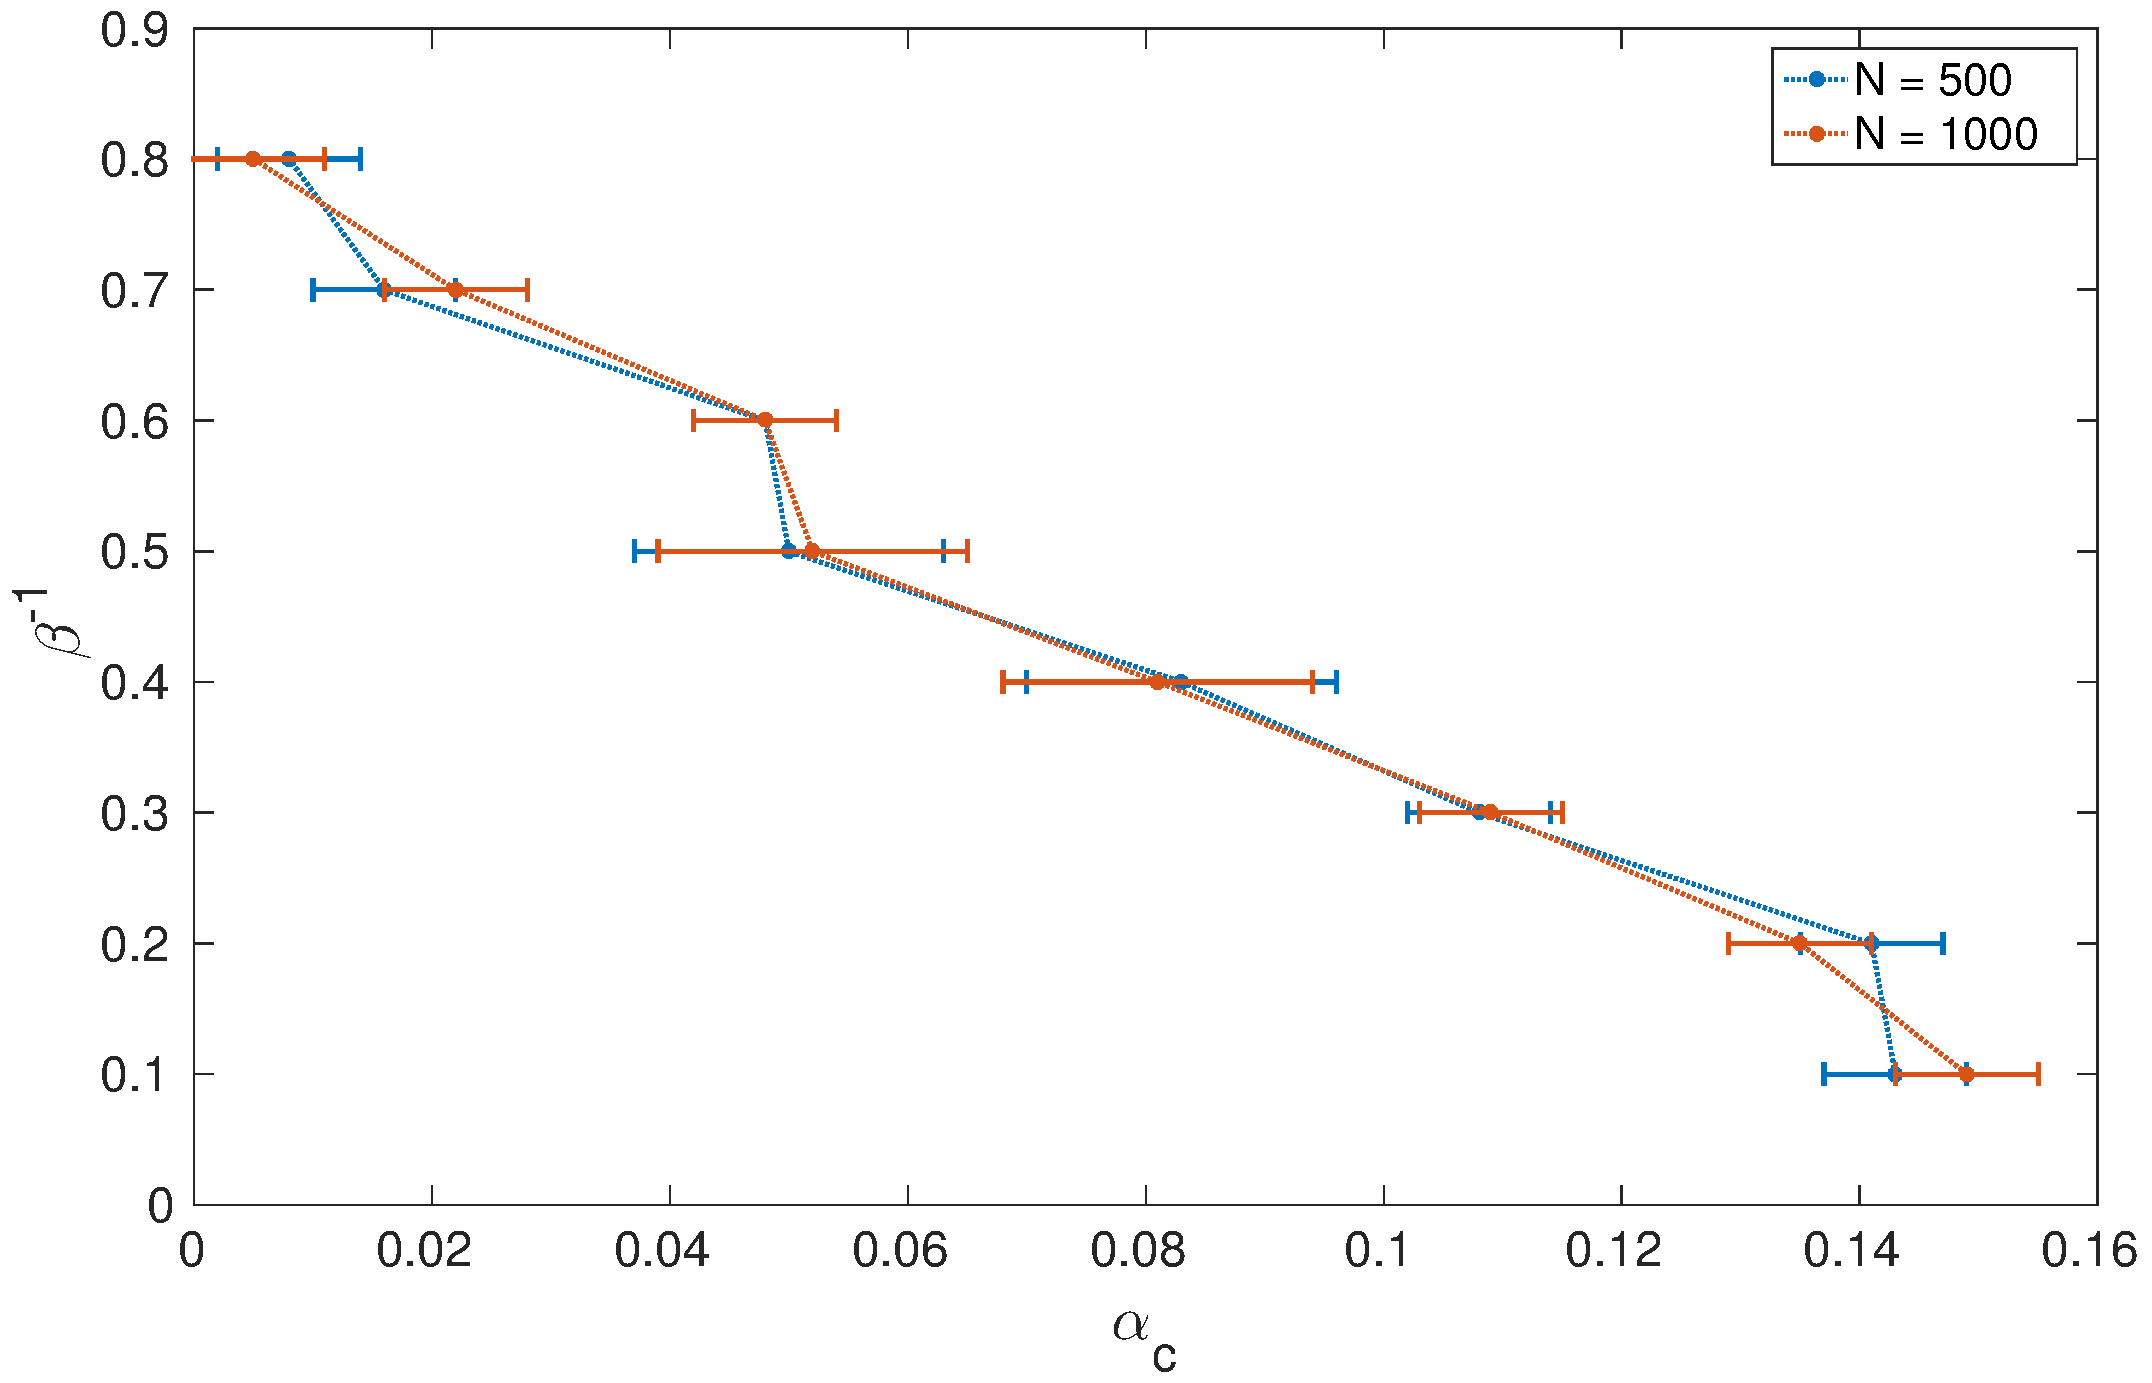
\includegraphics[width=\textwidth]{figures/fig_3b.pdf}
\caption{Critical values $\alpha_c$ (x-axis) as a function of $\beta^{-1}$ (y-axis) in a stochastic Hopfield network with either $N = 500$ bits (blue dots) or $N = 1000$ bits (red dots).}
\label{3b}
\end{figure}

Using the values in Table \ref{table1} and \ref{table2}, for each value of $N$ and $\beta^{-1}$ the couple of values ($\alpha_1$,$\alpha_2$) corresponding to the largest drop of $\left<m_1\right>$ were identified (e.g. for $N = 500$ and $\beta^{-1} = 0.1$, the interval of interest is $[\alpha_1$,$\alpha_2] = [0.125,0.15]$).
Then, for each such interval, additional simulations were run, for 3 more equally spaced values of $\alpha$ inside interval $[\alpha_1$,$\alpha_2]$, acquiring average values of $\left<m_1\right>$ in equilibrium ($1\cdot10^6$ updates, burn-in of $5\cdot10^5$). 

The resulting set of 5 values $\left<m_1(\alpha)\right>$ were used for a spline interpolation, to find the value $\alpha^*$ corrsponding to to $\left<m_1(\alpha^*)\right> = 0.5$. This value is our estimate of $\alpha_c(\beta^{-1})$, and the difference between two consecutive sampled (and \emph{not} interpolated) values of $\alpha$ is used as statistical error.

The resulting curves $\alpha_c(\beta^{-1})$ in Fig.~\ref{3b} roughly reflect the shape of the phase diagram of the stochastic Hopfield model, and this is the reason why $\alpha$ was kept on the x-axis and $\beta$ on the y-axis in this plot. 

However, a much larger network size $N$ and longer simulation runtime (which would allow, for instance, to be able to acquire uncorrelated MCMC samples for the order parameter) are required to give better estimates of $\alpha_c$.

\subsubsection*{Reference code}
See \textsc{matlab} script \verb!Exercise_3b.m! and custom functions called in the script itself.
\clearpage

\appendix
\section*{Appendix: MATLAB code}

\subsection*{\texttt{Exercise1a.m}}
\begin{lstlisting}
%EXERCISE1A
clear
clc
tic

% ======================================================= %
% Parameters
% ======================================================= %

nBits = 50;
nPatterns = 10;
nSamples = 4000;

% ======================================================= %

% Initializations
crossTalkTerms = zeros(nBits, nPatterns, nSamples);

% Main loop
h = waitbar(0, 'Please wait...');
for sample = 1:nSamples
    
    randomPatterns = GenerateRandomPatterns( nBits, nPatterns );
    crossTalkTerms(:,:,sample) = ComputeCTT(randomPatterns);
    
    waitbar(sample/nSamples,h);
end
close(h);

[h1 , f1] = PrettyPlotCTT(crossTalkTerms(:), nPatterns/nBits);
[h2 , f2] = LogPlotCTT(crossTalkTerms(:), nPatterns/nBits);
toc
\end{lstlisting}

\subsection*{\texttt{Exercise1b.m}}
\begin{lstlisting}
%EXERCISE1B
clear
clc
tic

% ======================================================= %
% Parameters
% ======================================================= %

nBits = 100;
nSamples = 10000;
maxNPatterns = 100;
patternID = 1; % first pattern by default
bitID = 1; % first bit by default

% ======================================================= %

[errorProbs] = CheckBitStability( nBits, maxNPatterns, nSamples, patternID, bitID );

% plot estimated probabilities
alpha = (1:maxNPatterns)/maxNPatterns;
plot(alpha,errorProbs,'bo');
hold on

% plot theoretical error probabilities
theorVals = 1/2*(1-erf(sqrt(1./(2.*alpha))));
plot(alpha,theorVals,'r');
hold off

% plot settings
set(gcf,'color','w')
xlabel('\alpha = p/N');
ylabel('P_{err}');
pbaspect([1.618 1 1]);
set(gca,'fontsize', 24);
toc
\end{lstlisting}

\subsection*{\texttt{Exercise2a2b.m}}
\begin{lstlisting}
%EXERCISE_2A_2B
clear
clc
tic

% ======================================================= %
% Parameters
% ======================================================= %

nBits = 500;
nPatterns = 100;
noise = 0.5;
tMax = 50000;
nRuns = 1;
patternID = 1;

% ======================================================= %

% Initializations
orderParams = zeros(nRuns,tMax);
fig = figure;

% Preliminary operations
beta = 1/noise;
randomPatterns = GenerateRandomPatterns( nBits, nPatterns );
weightMatrix = SetHebbsWeights( randomPatterns );
storedPattern = randomPatterns(:,patternID); 

for jj = 1:nRuns
    
    % Re-initialise network at each run
    networkState = randomPatterns(:, patternID);
   
    message = ['Please wait... Run ' num2str(jj) ' of ' num2str(nRuns)];
    h = waitbar(0, message);
    
    for tt = 1:tMax
    
    	% compute order parameter
    	orderParams(jj,tt) = ComputeOrderParam(storedPattern, networkState);

    	% update network
    	networkState = StochasticAsyncUpdate( networkState, weightMatrix, beta );

    	waitbar(tt/tMax,h);
       
    end
    close(h);
    
    figure(fig);
    plot(orderParams(jj,:),'LineWidth',1);
    hold on;
    
end

% Plot settings
set(gcf,'color','w');
f1 = plot(nan); 
f2 = plot(nan); 
f3 = plot(nan); 
f4 = plot(nan); 
f5 = plot(nan);
legend([f1,f2,f3,f4,f5],'Run 1', 'Run 2', 'Run 3', 'Run 4', 'Run 5')
pbaspect([1.618 1 1])
hold off;
toc
\end{lstlisting}

\subsection*{\texttt{Exercise3a.m}}
\begin{lstlisting}
%EXERCISE3A
clear 

% ======================================================= %
% Parameters
% ======================================================= %

noiseMax = 8; % using integer because of parfor loop
nBits = 500; % use 500 and 1000
nSweeps = 10000;
patternID = 1; % pattern to feed
alphaValues = [0.025, 0.05, 0.1, 0.125, 0.15, 0.2];
burnIn = 1000;

% ======================================================= %

% Initializations
orderParamDataset = zeros(noiseMax,length(alphaValues),nSweeps);
alphaID = 1;

h = waitbar(0, 'Please wait...');

for alpha = alphaValues
    tic

    % compute number of patterns according to alpha
    nPatterns = fix(nBits*alpha);

    % initialize local variable to temporary store m values
    orderParams = zeros(noiseMax,nSweeps);

    % parallel loop over noise
    parfor noise = 1:noiseMax

        beta = 10/noise;

        % generate random patterns and set weigths
        randomPatterns = GenerateRandomPatterns( nBits, nPatterns );
        weightMatrix = SetHebbsWeights( randomPatterns );

        % Feed network with pattern # patternID (default 1)
        networkState = randomPatterns(:, patternID);
        % and define pattern to compare with the network state
        storedPattern = randomPatterns(:,patternID); 

        for sweep = 1:nSweeps % run MCMC sweeps

            for tt = 1:nBits % and in each sweep update the network nBits times
                             % (so that on average each bit is updated once)
                networkState = StochasticAsyncUpdate( networkState, weightMatrix, beta );
            end

            % then compute and store order parameter
            orderParams(noise,sweep) = ComputeOrderParam(storedPattern, networkState);
        end
    end

    % finally store order parameter samples in an outer 3D array
    orderParamDataset(:,alphaID,:) = orderParams;
    alphaID = alphaID +1;
    
    waitbar(alphaID/length(alphaValues),h);
    toc
end
close(h);

% smoothing
for ii = 1:noiseMax
    for jj = 1:length(alphaValues)
        orderParamDataset(ii,jj,:) = smooth(squeeze(orderParamDataset(ii,jj,:)),100);
    end
end

% remove initial values (burnin)
dataset = dataset(:,:,burnIn+1:end);

meanValues = (mean(dataset,3));
lowerQuantiles = (quantile(dataset,0.05,3));
upperQuantiles = (quantile(dataset,0.95,3));
errors = max(upperQuantiles-meanValues,meanValues-lowerQuantiles);
\end{lstlisting}

\subsection*{\texttt{Exercise3b.m}}
\begin{lstlisting}
%EXERCISE3B
clear 
tic

% ======================================================= %
% Parameters
% ======================================================= %

noise = 0.1; % depending on this value, set alpha values below
howManyPoints = 5; % points to sample and then use for interpolation
alphaValues = linspace(0.125,0.15,howManyPoints); % alpha window of interest found in previous exercise (DEPENDS on noise!!)
nBits = 500; % use 500 and 1000
nSweeps = 1000;
patternID = 1; % pattern to feed
burnIn = 500;

% ======================================================= %

% Initializations
orderParamDataset = zeros(length(alphaValues),nSweeps);
beta = 1/noise;

parfor alphaID = 1:howManyPoints
    
    alpha = alphaValues(alphaID);
    % compute number of patterns according to alpha
    nPatterns = max(1,fix(nBits*alpha));

    % generate random patterns and set weigths
    randomPatterns = GenerateRandomPatterns( nBits, nPatterns );
    weightMatrix = SetHebbsWeights( randomPatterns );

    % Feed network with pattern # patternID (default 1)
    networkState = randomPatterns(:, patternID);
    % and define pattern to compare with the network state
    storedPattern = randomPatterns(:,patternID); 

    for sweep = 1:nSweeps % run MCMC sweeps

        for tt = 1:nBits % and in each sweep update the network nBits times
                         % (so that on average each bit is updated once)
            networkState = StochasticAsyncUpdate( networkState, weightMatrix, beta );
        end

        % then compute and store order parameter
        orderParamDataset(alphaID,sweep) = ComputeOrderParam(storedPattern, networkState);
    end
    
end

% remove initial values
nchorderParamDataset = orderParamDataset(:,burnIn+1:end);

% compute mean values
meanOrderParam = mean(orderParamDataset,2);

% interpolation
xq = linspace(min(alphaValues),max(alphaValues),5*howManyPoints);
vq2 = interp1(alphaValues,meanOrderParam,xq,'spline');
tmp = abs(vq2-0.5);
[val , idx] = min(tmp);

alphaCrit = xq(idx)
error = alphaValues(2)-alphaValues(1)

toc
\end{lstlisting}

\subsection*{Additional subroutines}

\bigskip
\begin{lstlisting}
function [ randomPatterns ] = GenerateRandomPatterns( nBits, nPatterns )

if nargin < 2
    nPatterns = 1;
end

randomPatterns = 2*round(rand(nBits,nPatterns))-1;

end
\end{lstlisting}

\bigskip

\bigskip
\begin{lstlisting}
function [ crossTalkTerms ] = ComputeCTT( patterns )
%COMPUTECTT

nBits = size(patterns,1);
nPatterns = size(patterns,2);
crossTalkTerms = zeros(size(patterns));

muVals = 1:nPatterns;

for k= 1:nBits

    %create temp matrix without j-th row (logical indexing for performance)
    index = true(1, size(patterns, 1));
    index(k) = false;
    tempMatrix = patterns(index,:);
    
    for nu = 1:nPatterns
        
        % allowed values of mu (all but mu=nu)
        allowedMus = muVals(muVals~=nu);
        
        for mu = allowedMus
            crossTalkTerms(k,nu) = crossTalkTerms(k,nu) + ...
                patterns(k,mu)*sum(tempMatrix(:,nu).*tempMatrix(:,mu));
        end
    end
end

% do not forget to multiply element-wise and divide by N
crossTalkTerms = -1/nBits*(crossTalkTerms.*patterns);
end
\end{lstlisting}

\bigskip

\bigskip
\begin{lstlisting}
function [ histHandle, curveHandle ] = PrettyPlotCTT( crossTalkTerms , alpha)
%PRETTYPLOTCTT
%   Remember that alpha = p/N

figure('units','normalized','outerposition',[0 0 1 1])

% plot histogram
histHandle = histogram(crossTalkTerms(:),16,'Normalization','pdf');
%histHandle.NumBins = round(histHandle.NumBins/20);

% create linspaced x values for normal curve
xVals = linspace( min(-2,min(crossTalkTerms(:))), max(2,max(crossTalkTerms(:))), 100);
yVals = normpdf(xVals, 0, sqrt(alpha));

% plot curve
hold on
curveHandle = plot(xVals,yVals,'r','LineWidth',2);
hold off

% additional settings
set(gcf,'color','w');
xlabel('C_k^{(\nu)}');
ylabel('-log P(C_k^{(\nu)})');
axis square;
set(gca,'fontsize', 30);

end
\end{lstlisting}

\bigskip

\bigskip
\begin{lstlisting}
function [ histHandle, curveHandle ] = LogPlotCTT( crossTalkTerms , alpha)
%LOGPLOTCTT
%   Remember that alpha = p/N

figure('units','normalized','outerposition',[0 0 1 1])

% create and plothistogram
%[binnedVals] = histcounts(crossTalkTerms(:));
%nBins = round(length(binnedVals)/23);
[estimatedProb,edges] = histcounts(crossTalkTerms(:),16,'Normalization','pdf');
binCenters = edges(1:end-1)+0.5*(edges(2)-edges(1));
histHandle = bar(binCenters,-log(estimatedProb));
hold on

% create normal curve points and plot them
xVals = linspace( min(-2,min(crossTalkTerms(:))), max(2,max(crossTalkTerms(:))), 100);
yVals = normpdf(xVals, 0, sqrt(alpha));
curveHandle = plot(xVals,-log(yVals),'r','LineWidth',2);
hold off

% plot settings
set(histHandle,'FaceColor', [0 0.4470 0.7410]);
set(gcf,'color','w');
xlabel('C_k^{(\nu)}');
ylabel('-log P(C_k^{(\nu)})');
axis square;
set(gca,'fontsize', 30);

end
\end{lstlisting}

\begin{lstlisting}
function [errorProbs] = CheckBitStability( nBits, maxNPatterns, nSamples, patternID, bitID )
%CHECKBITSTABILITY

% initialize 2D logical array of errors
boolErrors = false(maxNPatterns,nSamples);

h = waitbar(0,'Please wait...');

for nPatterns = 1:maxNPatterns % run over different p/N ratios
    
    parfor ii = 1:nSamples

        % generate nPatterns new random patterns and train network
        randomPatterns = GenerateRandomPatterns( nBits, nPatterns );
        weightMatrix = SetHebbsWeights(randomPatterns);

        % feed pattern # patternID and check stability of bit # bitID
        outputPattern = DeterministicSyncUpdate(randomPatterns(:,patternID),weightMatrix);
        if outputPattern(bitID,patternID) ~= randomPatterns(bitID,patternID)
            boolErrors(nPatterns,ii) = true;
        end
    end

    waitbar(nPatterns/maxNPatterns,h)
end
close(h);

errorProbs = mean(boolErrors,2); % average over samples

end
\end{lstlisting}

\bigskip

\bigskip
\begin{lstlisting}
function [ weightMatrix ] = SetHebbsWeights( patterns )
%SETHEBBSWEIGHTS

nBits = size(patterns,1);

% compute W matrix in a smart way
weightMatrix = 1/nBits*(patterns*patterns');

% set diagonal elements to zero
weightMatrix(logical(eye(size(weightMatrix)))) = 0;

end
\end{lstlisting}

\bigskip

\bigskip
\begin{lstlisting}
function [ orderParam ] = ComputeOrderParam( storedPattern, networkState )
%COMPUTEORDERPARAM

orderParam = 1/length(storedPattern)*(storedPattern'*networkState);

end
\end{lstlisting}

\bigskip

\bigskip
\begin{lstlisting}
function [ newNetworkState ] = DeterministicSyncUpdate( networkState, weightMatrix )
%DETERMINISTICSYNCUPDATE

newNetworkState = sign(weightMatrix*networkState);
% ...as easy as that!

end
\end{lstlisting}

\bigskip

\bigskip

\begin{lstlisting}
function [ newNetworkState ] = StochasticAsyncUpdate( networkState, weightMatrix, beta )
%STOCHASTICASYNCUPDATE

% Pick bit to update uniformly at random
nBits = length(weightMatrix);
ii = randi(nBits);

% Evaluate Boltzmann factor
b_ii = weightMatrix(ii,:)*networkState;
boltz = 1/(1+exp(-2*beta*b_ii));

% Update bit i
newNetworkState = networkState;
if rand() < boltz
    newNetworkState(ii) = +1;
else
    newNetworkState(ii) = -1;
end

end
\end{lstlisting}

\end{document}
